\documentclass[12pt,a4paper]{article}
\usepackage[utf8]{inputenc}
\usepackage[british]{babel}
\usepackage[autostyle]{csquotes}
\usepackage{amsmath, amsfonts, amssymb, array, amsthm}
\usepackage{graphicx, subcaption}
%\captionsetup{justification=centering}
\usepackage{setspace}
\usepackage{multicol}
\usepackage{parskip}
\setlength{\parindent}{3em}
\usepackage{fancyhdr}
\usepackage{hyperref}
\usepackage{pgfplots}
\pgfplotsset{compat=newest}% use newest version
\usepackage{tikz, tikz-3dplot,  circuitikz}
\usetikzlibrary{matrix,chains,positioning,decorations.pathreplacing,arrows,plotmarks, calc, intersections}
\usepackage{xcolor} % text colours
\usepackage{sectsty} % style sections
\usepackage{xstring}
\usepackage{caption}
\usepackage{listings} % source code formatting
\usepackage[natbib=true, style=phys, sorting=none]{biblatex} % bibliography
\addbibresource{citations.bib} 
\addbibresource{IOPEXPORT.bib}
\usepackage{notoccite}
\usepackage{setspace}
\usepackage{wrapfig}
\usepackage{mathrsfs}
\usepackage[tmargin=1in,bmargin=1in,lmargin=1.25in,rmargin=1.25in]{geometry}


\title{Generating Molecules with Machine Learning}
\date{2020\\ March}
\author{Oisín Peppard\thanks{Supervised by Dr. Stefano Sanvito}\thanks{Mentorship from James Nelson}}

% Define colours
\definecolor{blu2}{HTML}{206B99}
\definecolor{plumb}{HTML}{A16E83}
\definecolor{pink1}{HTML}{E18AAA}
\definecolor{gren}{HTML}{B4D3B2}
\definecolor{pink2}{HTML}{DA7B93}
%%%%%%%%%%
\definecolor{blu1}{HTML}{5DA2D5}
\definecolor{lightblu}{HTML}{90CCF4}
\definecolor{red1}{HTML}{F78888} %#ecb4b4
\definecolor{red2}{HTML}{EDB5BF}
\definecolor{lilacc}{HTML}{86B3D1}
\definecolor{gren1}{HTML}{b4ecb4}
\definecolor{gren2}{HTML}{73dc73}
%%%%%%%%%%
\hypersetup{colorlinks=true, linkcolor=blu2, urlcolor=plumb, filecolor=blu2, citecolor=plumb}

% Title and Subtitle
\newcommand{\Title}[1]{\begin{center}\textcolor{blu2}{\begin{Huge}#1\vspace{12pt}\end{Huge}}\end{center}}
\newcommand{\SubTitle}[1]{\begin{center}\textcolor{blu2}{#1\vspace{20pt}}\end{center}}

% Color of Headings
\subsectionfont{\color{blu2}}
\sectionfont{\color{plumb}}
\subsubsectionfont{\color{plumb}}

% Line spacing
\linespread{1.3} %1.5 spacing

% For quoting code
\lstdefinestyle{Oisins}{
    backgroundcolor=\color{white},   
    commentstyle=\color{blu2},
    keywordstyle=\color{plumb},
    numberstyle=\tiny\color{gray},
    stringstyle=\color{pink1},
    basicstyle=\scriptsize\ttfamily,breaklines=true,
    breakatwhitespace=false, 
    xleftmargin=20pt, 
    xrightmargin=20pt,       
    breaklines=true,                 
    captionpos=b,                    
    keepspaces=true,                 
    numbers=left,                    
    numbersep=5pt,                  
    showspaces=false,                
    showstringspaces=false,
    showtabs=true,                  
    tabsize=2,
    framextopmargin=50pt,
    frame=bottomline,
    language=Python,
    numberblanklines = false
}
\lstset{style=Oisins}

% Header
%     \pagestyle{fancy}
 %    \fancyhf{}
  %   \rhead{Right Header}
   %  \lhead{Left Header}
    % \cfoot{\thepage}
     %\thispagestyle{plain}

\begin{document}

\begin{figure}
    \centering
    \includegraphics[width = 0.75\linewidth]{images/logo.jpg}
\end{figure}

\vspace{5cm}
\Title{Generating Molecules with Machine Learning}
\SubTitle{Oisín Peppard}
\SubTitle{March 2020}
\SubTitle{Supervised  by Dr. Stefano Sanvito \\ Mentored by James Nelson}
% \maketitle
\begin{abstract}
\noindent
\centering
In this project, numerical algorithms and machine learning methods were implemented, with their suitability explored in the context of generating molecules. Neural networks were successfully used to predict energies of hypothetical 2-D trigonal molecules, with mean average error of 0.12\%. GANs were used to reproduce distributions of molecules and as such, create \emph{\enquote{fake}} molecules indistinguishable from the real. The methods examined here have potential applications in the generation of new materials with desired properties.
\end{abstract}
\pagebreak
\linespread{0.9}{% spacing for ToC
\small{\tableofcontents}}
\linespread{1.3}% back to 1.5 spacing
\pagebreak
\section{Introduction}
%The motivation for this study came from a review published in \enquote{Science} highlighting the advantages of using Machine learning to accelerate the discovery of new chemical compounds \cite{sanchez-lengeling_inverse_2018}. 
The discovery of new materials can effect momentous societal advancement. Indeed many contemporary issues stem from physical limitations of materials, such as a conventional \emph{silicon} solar cells' limitation to 25\% power conversion efficiency holding back renewable energy \cite{green_corrigendum_2017}. Historically, synthesis of new materials was a slow process that required many steps, frequently taking up to 20 years in total \cite{maine_commercializing_2006}. Often, new materials come from a crude method of trial and error, and many important materials were discovered by chance, (including the likes of Teflon, anaesthetic and Vaseline \cite{sanchez-lengeling_inverse_2018}). One such story is that of Perkin’s mauve.

In 1856, an eighteen year old chemist was attempting to synthesise quinine as a treatment for malaria, but in an unsuccessful attempt, happened upon a dye that transformed the textile industry \cite{prisco_color_2017}. Another famous example is the discovery of penicillin. Sir Alexander Fleming mistakenly left his staphylococcus culture near an open window for a fortnight, and returned to find a mould that halted its growth - thus discovering the world's first antibiotic \cite{markel_real_2013}. 

In 2014, it was reported that 49\% of cancer treatment drugs were made from natural products or their derivatives \cite{cragg_natural_2016}. Clearly, modern society is heavily dependent on these \emph{discoveries}, and could benefit greatly from a more efficient, direct \emph{design} of new materials and chemicals. Future materials could potentially come from unexplored regions of chemical space: the set of all synthetically feasible organic molecules. \enquote{The Chemical Space Project} \cite{reymond_chemical_2015} has catalogued 166.4 billion molecules with up to 17 heavy atoms, although the actual number of potential structures is estimated to be of the order $10^{60}$ \cite{virshup_stochastic_2013}. Direct exploration of chemical space is a Sisyphean task, but machine learning is a promising candidate for smart navigation. As suggested by Sanchez-Lengeling in his article in \enquote{Science}:
\begin{quote}
    \enquote{\emph{The ultimate aim is to concurrently propose, create, and characterise new materials, with each component transmitting and receiving data simultaneously} \cite{sanchez-lengeling_inverse_2018}.}
\end{quote}
In 1961, Donald Michie was an artificial intelligence researcher at Bletchley Park \cite{noauthor_obituary_2007}. Here, he developed the Machine Educable Noughts And Crosses Engine (MENACE) \cite{michie_experiments_1963}. This project was one of the earliest examples of self updating algorithm, and is a simple and elegant idea to begin a foray into machine learning. MENACE consisted of 304 matchboxes, each representing one of the unique noughts and crosses board states. Boxes  were filled with coloured beads representing different moves, with the number of beads of a given colour indicative of that move's probability of leading to a win. The program was trained by playing a game, with random beads taken from each appropriate box dictating the next move \cite{michie_experiments_1963}, and beads that lead to a loss removed at the end. After about 250 games, MENACE is trained to draw or win every game. This simplistic algorithm was a seminal implementation of what would become the cornerstone of 21st century machine learning - reinforcement learning via a feedback loop.

In this project, we aim to explore the capabilities and challenges of some modern machine learning methods in generating molecules. We will use neural networks to predict molecule energies, and Generative adversarial networks to create new ones. We will look at optimal representation of training data, and processing of data that optimises machine learning performance.

\section{Theory and Background}
\subsection{Supervised Machine Learning} \label{subsec:sml}
In machine learning (ML), the goal is for a program to approximate, or \emph{learn} a function $f: \textbf{X} \to Y$. An input, usually referred to as the feature vector, is drawn from $\textbf{X}$ and mapped by to a target variable $Y$ \cite{goodfellow_deep_2016}. Neural networks (NN) are the canonical example of an algorithm that exhibits machine learning, and what were employed throughout this project. The output of the network is denoted $\hat{y}$,the goal is to get this close to  $y \in Y$. 

\emph{Supervised} ML means that input data comes with a label, or a predetermined result that we are trying to replicate. This is counter to \emph{unsupervised} learning, where a computer program seeks hidden structure in data; trends and correlations that are not known before training. There are two main subcategories of supervised ML.
\begin{itemize}
    \item \textbf{Regression} is the process of reproducing a given function \cite{goodfellow_deep_2016} e.g. \textit{given a molecular shape $\in \textbf{X}$, what is its energy?}
    \item \textbf{Classification} seeks to determine if an element in $\textbf{X}$ belongs to a given category \cite{goodfellow_deep_2016}. Here the target variable is a vector with dimension equal to the number of categories to be sorted into. e.g. \emph{given a molecule, what properties will it have?} A special case of this is binary classification. Here the feature vector consists of two categories and can be represented by a single Boolean bit. \emph{Is a given molecule stable (1) or unstable (0)?}
\end{itemize}{}
Training a NN begins by splitting training data into three disjoint sets: training, validation and test \cite{goodfellow_deep_2016}. The network's output can be written \begin{equation}
    \hat{y}=f(\mathbf{x}; \theta, \lambda),
\end{equation}
where $\theta$ represents model parameters learned with the \emph{training set}. The purpose of $\lambda$, denoting the hyperparameter, is to correct overfitting, a phenomenon illustrated in figure \ref{fig:overfitting}. These parameters are optimised by training on the \emph{validation set}, data the network has not yet seen but uses to tweak predictions. In order to train a network, we define a loss function\cite{goodfellow_deep_2016} 
\begin{equation}
L(y,\hat{y}) \quad y \in \textbf{Y} \quad \hat{y} \in f(\textbf{X}),
\end{equation}
which is some measure of how much a prediction $\hat{y}$ from $f$ differs from the true value $y$ in the target training data. The training process should aim to minimise this. We also define a cost function $J(\theta,\lambda)$ for both training and validation sets. This is generally the average loss of each datum in the relevant training set, with some penalty term to prevent overfitting\footnote{Definitions for $L$ and $J$ vary, and are often used interchangably. Usually $L$ is for error in a single prediction, while $J$ is for error over a whole set.}. By minimising these $J$ with respect to their implicit variables, the function updates its parameters and \emph{\enquote{learns}} to make better predictions. Its predictions are tested on the test set and used to evaluate its performance.
%%%%%  overfitting  pic  %%%%%%
\begin{figure}[h!]
    \centering
    \begin{tikzpicture}[font=\sffamily,
    declare function={f(\x)=0.5*pow(abs(\x-2),2)-0.06*pow(\x-2,3);}]
     \foreach \Z in {1,...,42}
     {\pgfmathsetmacro{\X}{\Z/10}
     \pgfmathsetmacro{\Y}{f(\X)+0.9*rnd}
     \ifnum\Z=1
      \xdef\LstOne{(\X,\Y)}
      \xdef\LstTwo{"(\X,\Y)"}
     \else
      \xdef\LstOne{\LstOne (\X,\Y)}
      \xdef\LstTwo{\LstTwo,"(\X,\Y)"}
     \fi}
     \begin{scope}[local bounding box=over,xshift=-5cm]
     \foreach \Z in {1,...,40}
     {\pgfmathsetmacro{\Last}{{\LstTwo}[\Z-1]}
     \pgfmathsetmacro{\Current}{{\LstTwo}[\Z]}
     \pgfmathsetmacro{\Next}{{\LstTwo}[\Z+1]}
    %\typeout{\Last,\Current,\Next} % was commented
      \edef\temp{\noexpand\path ($0.6*\Current+0.2*\Last+0.2*\Next$)   coordinate 
      (p\Z);}
      \temp
      \ifnum\Z=1
      \xdef\LstThree{(p\Z)}
      \else
      \xdef\LstThree{\LstThree (p\Z)}
      \fi
      }
     \foreach \Z in {1,...,42}
     {\pgfmathsetmacro{\Coor}{{\LstTwo}[\Z-1]}
     \fill \Coor circle[radius=1pt];
     }
     \draw[thick,plumb] plot[smooth] coordinates \LstThree;
%     \caption{Underfitting}
    % \node [below = 1cm of over] {\parbox{0.3\linewidth}{\subcaption{Overfitting}\label{subfig:c}}};
     \end{scope}
     %
     \begin{scope}[local bounding box=good,xshift=-10cm]
     \foreach \Z in {1,...,42}
     {\pgfmathsetmacro{\Coor}{{\LstTwo}[\Z-1]}
     \fill \Coor circle[radius=1pt];
     }
     \draw[thick,plumb] plot[smooth,domain=0.1:4.2,variable=\x] (\x,{f(\x)+0.45});
     %\node [below =1cm of good] {\parbox{0.3\linewidth}{\subcaption{Good fit}\label{subfig:b}}};
%     \caption{Good fit}
     \end{scope}
     %
     \begin{scope}[local bounding box=under,xshift=-15cm]
     \foreach \Z in {1,...,42}
     {\pgfmathsetmacro{\Coor}{{\LstTwo}[\Z-1]}
     \fill \Coor circle[radius=1pt];
     }
     \draw[thick,plumb] (0.1,0.4) -- (4.2,2);
     %\node [below = 1cm of under] {\parbox{0.3\linewidth}{\subcaption{Underfitting}\label{subfig:a}}};
%     \caption{Overfitting}
     \end{scope}
     %
     \foreach \X in {over,good,under}
     {\draw[gray,thin] ([xshift=-3pt,yshift=3pt]\X.north west) rectangle 
     ([xshift=3pt,yshift=-3pt]\X.south east);
     \draw[stealth-stealth,thick] ([xshift=-3pt,yshift=3pt]\X.north west) node[right=1.5pt,fill=white]{Values} 
     |- ([xshift=3pt,yshift=-3pt]\X.south east) node[below left]{Time};}
     \node [below = of under] {\parbox{0.3\linewidth}{\subcaption{Underfitting}\label{subfig:a}}};
     \node [below = of good] {\parbox{0.3\linewidth}{\subcaption{Good fit}\label{subfig:b}}};
     \node [below = of over] {\parbox{0.3\linewidth}{\subcaption{Overfitting}\label{subfig:c}}};
\end{tikzpicture}
\caption{Neural network learning outcomes. The first case (\ref{subfig:a}) is underfitting, where the network has not learned any correlation in the data. The second case (\ref{subfig:b}) is a good fit, whereby the network has learned the underlying pattern which we want to replicate. The third case (\ref{subfig:c}) is overfitting. The network finds and learns patterns in the training data but does not learn the overall desired function, the performance criterion will evaluate the network to be making good predictions since it hits all training data, but in reality, It is incorrect. Hyperparameters optimised on the validation set are used to remedy this.}
\label{fig:overfitting}
\end{figure}
\pagebreak
\subsection{GAN} \label{subsec:gan}
Generative Adversarial Networks \cite{goodfellow_generative_2014} are a revolutionary method for neural networks to generate original data. A simple project entitled \href{https://thispersondoesnotexist.com}{\enquote{This Person Does Not Exist}} \cite{karras_et_al._this_2019} is a remarkable display of how powerful this technology is. A general principle of artificial intelligence, is that it is far easier for a computer to \emph{learn} something about given data, than it is to \emph{create} such data itself. 

\begin{quote}
\emph {\enquote{What I cannot create, I do not understand}}
  \begin{flushright}
    \footnotesize{\textbf{---Richard P. Feynmann}}
  \end{flushright}
\end{quote}
The idea is to employ two neural networks in an adversarial manner. One is the generator, hereafter referred to as $G$. The other is the Discriminator, $D$. A common analogy is that of $G$ as a counterfeiter trying to create fake data indistinguishable from its training data, while $D$ is akin to a detective trying to identify if a given sample is \emph{real}, or a \emph{fake} generated by $G$ \cite{goodfellow_generative_2014}. $D$ and $G$ are trained simultaneously until $D$ is unable to distinguish between real and fake data. At this point (if both are trained correctly), $G$ is a competent generator of artificial or \emph{fake} data. The process is outlined schematically in figure \ref{fig:gan}.
% GAN shematic
\begin{figure}[ht]
        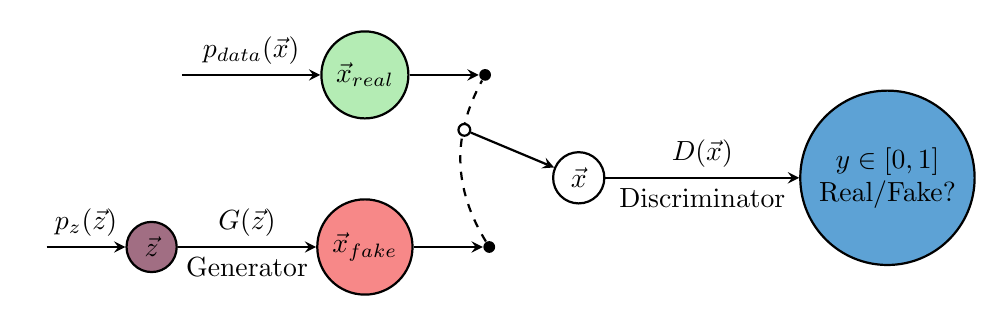
\begin{tikzpicture}

	\node[circle, draw, thick, fill=plumb] (z) {$\vec{z}$};
	\node[circle, draw, thick, right=5em of z, fill = red1] (x) {$\vec{x}_{fake}$};
	\draw[-stealth, thick ] (z) -- node[above] {$G(\vec{z})$} node[below] {Generator} (x);
	\node[left=of z] (i) {};
	\draw[-stealth, thick ] (i) -- node[above] {$p_z(\vec{z})$} (z);
	\node[above=of x, circle, draw, thick, fill = gren1] (xt) {$\vec{x}_{real}$};
	\node[left=5em of xt] (it) {};
	\draw[-stealth, thick] (it) -- node[above] {$p_{data}(\vec{x})$} (xt) ;
	\node[circle, draw, thick, right=5em of x, yshift=2.5em] (D) {$\vec{x}$};
	\node[circle, draw,  thick, right=7em of D, fill = blu1, align=center] (out) {$y\in [0,1]$ \\ Real/Fake?};
	\draw[-stealth, thick] (D) -- node[above] {$D(\vec{x})$} node[below] {Discriminator} (out);
			
	\node[right=2.5em of x, circle, fill, inner sep=0.15em] (pt1) {};
	\node[right=2.5em of xt, circle, fill, inner sep=0.15em] (pt2) {};
			
	\draw[dashed, thick] (pt1) edge[bend left] (pt2);
			
	\node[circle, draw, thick, fill=white, inner sep=0.15em] at ([xshift=-0.9em, yshift=4em]pt1.north) (pt3) {};
			
	\draw[-stealth, thick] (x) -- (pt1);
	\draw[-stealth, thick] (xt) -- (pt2);
	\draw[-stealth, thick] (pt3) -- (D);

        \end{tikzpicture}
    \caption{Schematic diagram of a GAN. \emph{Real} data are drawn from the training dataset with a distribution $p_d(x)$. A neural network $G$ - the generator - creates \emph{fake} data from its input drawn from a latent distribution $p_z(z)$. Both real and fake data are passed through a second neural network $D$ - the discriminator - which outputs 0 if it believes the input to be fake, and 1 if it believes it real.}
    \label{fig:gan}
\end{figure}
\subsection{Three Atom Molecule}
In subsequent computational experiments, we simulate a generic homonuclear, three atom molecule in two dimensions. We approximate the molecular interaction with the Lennard-Jones (12,6) potential \cite{Lennard_Jones_1931} given in equation \ref{eq:LJ}. Here, $r_0$ is the distance between two nuclei that corresponds to a minimum in potential, $\epsilon$ is the depth of the potential well and $r$ is the distance between two atomic centres. 
\begin{equation}\label{eq:LJ}
    V_{LJ} = \epsilon \left[ \left(\frac{r_0}{r}\right)^{12} - 2 \left(\frac{r_0}{r}\right)^6 \right].
\end{equation}
For a multi atom molecule, configuration space will be a potential energy hypersurface (also called the Born-Oppenheimer surface) that describes the energy in terms of geometric position. Minima of this surface will correspond to a stable atomic configuration \cite{partay_efficient_2010}. In the following numerical  modelling parameters were chosen as $r_0=1$ and $\epsilon=10$ without units. The focus of this project is not realistic simulation, but to examine the ML methods, and so units are omitted for brevity. Qualitative results are obtained.

\section{Theoretical and Computational Method}
\subsection{Optimisation of Multilayer Perceptron Neural Networks}
A component of a neural network such as that discussed in section \ref{subsec:sml} is represented by 
\begin{equation} \label{eq:nn}
    \vec{\textbf{z}} = \mathbf{W} \cdot \vec{\mathbf{x}} + \vec{\textbf{b}}.
\end{equation}
 $\textbf{W}$ is a matrix of \emph{weights}, $\vec{\mathbf{x}}$ is the previous layer, and $\vec{\textbf{b}}$ is a vector containing \emph{biases}. Each element of the feature vector feeds to a layer of nodes called \emph{perceptrons}. This layer in turn feeds another layer of perceptrons, and this repeats for an arbitrary number of hidden layers until data has propagated through to the target variable. Each perceptron's input is a number with a \emph{weight} from each in the layer before, and a scalar bias can be added to increase or decrease its contribution to the overall output. Deep learning is a NN with more than one hidden layer. A schematic diagram of a neural network is given in figure \ref{fig:nn}, and detailed for a single perceptron in figure \ref{fig:perceptron}.

Since equation \ref{eq:nn} is a linear transformation, a network of such layers will itself only be capable of producing a linear transformations. Each perceptron output is passed through a non-linear \emph{activation function}, so it can model arbitrary functions. This means a neural network can approximate any Borel measurable function, as was proven by Hornik \cite{hornik_multilayer_1989}. Some activation functions are given in table \ref{tab:acfns}. NNs are inspired by neurons in the brain, which intake signal from several other neurons, light up some amount, then propagate signal.

\begin{table}[hb] 
    \centering
    \begin{tabular}{|l|l|} \hline
        ReLu - Rectified linear units & $\max (0,x)$                         \\%\hline
        Sigmoid                       & $ \left( 1+ e^{-x} \right  )^{-1}$  \\%\hline
        Hyperbolic Tangent              & $\tanh{x}$                        \\\hline
\end{tabular}
\caption{Most common neural network activation functions. In subsequent sections, ReLu is used, the output of the network to be jagged and not smooth.}
\label{tab:acfns}
\end{table}
%%%%%%%%%%%%%% NN Figure  %%%%%%%%%%%%%%%
\begin{figure}[h]
    \begin{subfigure}[t]{0.4\linewidth}
    \centering
    %\resizebox{0.5}{!}{%
    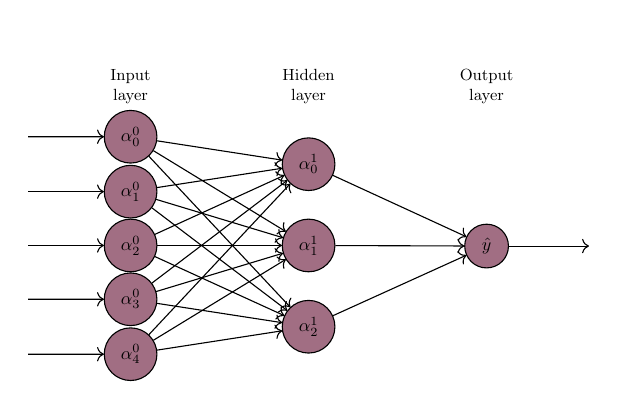
\begin{tikzpicture}[scale=0.65, 
        every node/.style={scale=0.65},
        %transform canvas={scale=0.7},
         % define styles 
          clear/.style={
          draw=none,
          fill=none,
          },
        net/.style={
          matrix of nodes,
          nodes={
               draw,
               circle,
               inner sep=5pt, %10
               fill=plumb
          },
          nodes in empty cells,
          column sep=1cm, %2
          row sep=-9.5pt, %-19
          } 
    ]
        % define matrix mat to hold nodes
        % using net as default style for cells
        \matrix[net] (mat)
        {
            % Define layer headings
            |[clear]| \parbox{1.3cm}{\centering \small Input layer} %1.3
              & |[clear]| \parbox{1.3cm}{\centering \small Hidden layer} 
              & |[clear]| \parbox{1.3cm}{\centering \small Output layer} \\
         
            $\alpha_{0}^{0}$  & |[clear]|        & |[clear]| \\
            |[clear]|         & $\alpha_{0}^{1}$ & |[clear]| \\
            $\alpha_{1}^{0}$  & |[clear]|        & |[clear]| \\
            |[clear]|         & |[clear]|        & |[clear]| \phantom{$\alpha_{0}^{0}$} \\
            $\alpha_{2}^{0}$  & $\alpha_{1}^{1}$ & $\hat{y}$ \\
            |[clear]|         & |[clear]|        & |[clear]|  \phantom{$\alpha_{0}^{0}$} \\
            $\alpha_{3}^{0}$  & |[clear]|        & |[clear]| \\
            |[clear]|         & $\alpha_{2}^{1}$ & |[clear]| \\
            $\alpha_{4}^{0}$  & |[clear]|        & |[clear]| \\ 
        };
        
        
        % left most lines into input layers
        \foreach \ai in {2,4,...,10}
            \draw[<-] (mat-\ai-1) -- +(-2cm,0);
        
        % lines from a_{i}^{0} to each a_{j}^{1}
        \foreach \ai in {2,4,...,10} {
            \foreach \aii in {3,6,9}
                \draw[->] (mat-\ai-1) -- (mat-\aii-2);
                }
        
        % lines from a_{i}^{1} to a_{0}^{2}
        \foreach \ai in {3,6,9}
          \draw[->] (mat-\ai-2) -- (mat-6-3);
            
        % right most line with Output label
        \draw[->] (mat-6-3) -- node[above] {} +(2cm,0); %3
        
    \end{tikzpicture}
    %}
    %\subcaption{Example of a feed-forward neural network architecture. Here the feature vector is four dimensional, there is one hidden layer, and a one dimensional target variable. Each perceptron is fed the output of each perceptron in the layer \emph{before} it until the data propagates from feature vector to output. Some networks employ backpropagation to transmit data to perceptrons in previous layers.}
    \caption{Neural network architecture}\label{fig:nn}
    \end{subfigure}\hspace{0.1\linewidth}%
    \begin{subfigure}[t]{0.3\linewidth}
    \centering
    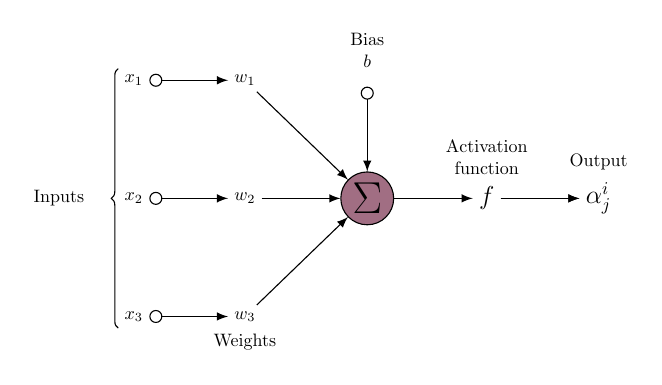
\begin{tikzpicture}[
        %scale=0.65, 
        every node/.style={scale=0.65},
        % define styles    
        init/.style={ 
             draw, 
             circle, 
             inner sep=2pt,
             font=\Huge,
             join = by -latex
        },
        squa/.style={ 
            font=\Large,
            join = by -latex
        }
    ]
        % Top chain x1 to w1
        \begin{scope}[start chain=1]
            \node[on chain=1] at (0,1.5cm)  (x1) {$x_1$};
            \node[on chain=1,join=by o-latex] (w1) {$w_1$};
        \end{scope}
        % Middle chain x2 to output
        \begin{scope}[start chain=2]
            \node[on chain=2] (x2) {$x_2$};
            \node[on chain=2,join=by o-latex] {$w_2$};
            \node[on chain=2,init,fill=plumb] (sigma) {$\displaystyle\Sigma$};
            \node[on chain=2,squa,label=above:{\parbox{2cm}{\centering Activation\\ function}}]   {$f$};
            \node[on chain=2,squa,label=above:Output,join=by -latex] {$\alpha_{j}^{i}$};
        \end{scope}
        % Bottom chain x3 to w3
        \begin{scope}[start chain=3]
            \node[on chain=3] at (0,-1.5cm) 
            (x3) {$x_3$};
            \node[on chain=3,label=below:Weights,join=by o-latex]
            (w3) {$w_3$};
        \end{scope}
        % Bias
        \node[label=above:\parbox{2cm}{\centering Bias \\ $b$}] at (sigma|-w1) (b) {};
        % Arrows joining w1, w3 and b to sigma
        \draw[-latex] (w1) -- (sigma);
        \draw[-latex] (w3) -- (sigma);
        \draw[o-latex] (b) -- (sigma);
        % left hand side brace
        \draw[decorate,decoration={brace,mirror}] (x1.north west) -- node[left=10pt] {Inputs} (x3.south west);
    \end{tikzpicture}
    \caption{\makebox[1pt][l] {Single perceptron}}\label{fig:perceptron}
    \end{subfigure}
\caption{\ref{fig:nn} is an example of a feed-forward neural network architecture. Here the feature vector is five dimensional, there is one hidden layer, and a one dimensional target variable. Each perceptron is fed the output of each perceptron in the layer \emph{before} it until the data propagates from feature vector to output. Some networks employ backpropagation to transmit data to perceptrons in previous layers. In \ref{fig:perceptron}, the operation of a single perceptron is shown. It receives input from each in the layer before it, with a corresponding weight. A bias is also added before it transmits to the next layer.}
\end{figure}
%%%%%%%%%%%%%%%%%%%%%%%%%%%%%%%%%%%%%%%%%
\pagebreak
The NN will naturally evolve to minimise loss until it reaches a state of overfitting. Here, loss will be very low since the function passes through every point of the training data, but it will not be the desired result. There are several techniques to overcome this. Some examples used in this project were:
\begin{itemize}
    \item \textbf{Simplifying} model complexity by manually removing layers or perceptrons
    \item \textbf{Early stopping} - stopping training when loss reaches a minimum threshold
    \item \textbf{Dropout} - randomly assigning a perceptron's parameters to zero during training iterations, and forcing the network to learn different paths.
    \item \textbf{Regularisation} - adding a hyperparameter term such as $\lambda \mathbf{w}^2$ to the cost function $J$. This essentially penalises the network's weights, so that minimising $J$ forces them to be smaller, and the network to be simpler. The optimal value of $\lambda$ is determined by testing on the validation set \cite{goodfellow_deep_2016}.
\end{itemize}
The general cost function for regression with regularisation becomes
\begin{equation}
    J(\theta, \lambda) = \frac{1}{N}  \sum^N L(y^{(i)},  f(\mathbf{x}^{i}; \theta)) + \lambda \textbf{w}^2.
\end{equation}
The Loss function used for regression in this project is mean squared error,
\begin{equation} \label{eq:mse}
    L(y,\hat{y}) = (y-\hat{y})^2.
\end{equation}
For binary classification, we use binary cross-entropy or log loss:
\begin{equation}
-y \log(\hat{y}) - (1-y)\log (1-\hat{y}),
\end{equation}
where $\hat{y} \in [0,1]$ is a probability of $y$ being in either of the two categories.

The next step is to minimise the cost function to find optimal choice of model parameters $\theta$ 
(representing all weights and biases) and $\lambda$. The computational method for this is determined by the \emph{optimiser}. Most optimisers are based on a form of gradient descent (see appendix \ref{app:gradient}). A common modfication to pure gradient descent is \emph{stochastic} gradient descent. This involves dividing training data into smaller batches, and updating parameters after cycling through a single batch\cite{goodfellow_deep_2016}. This is more efficient than cycling through the entire dataset. One cycle through the full dataset is called an \emph{epoch}. This is the natural timescale for a network's learning curve. A network will generally train over a few hundred epochs.
%do an appendix  on this https://towardsdatascience.com/understanding-binary-cross-entropy-log-loss-a-visual-explanation-a3ac6025181a
\subsection{GAN Training Criterion}
The training data, or \emph{real} data $\textbf{X}$ follows a distribution $p_d(x)$ for $x\in X$. The generator ($G$) creates \emph{fake} data with a distribution $p_g(z) = G(z;\theta_g)$. The vector $z$ is drawn from an arbitrary prior distribution $p_z(z)$, usually chosen to be a zero-centred, unit variance Gaussian. 

The goal for the GAN's training is for $p_g(z)$ to converge on $p_d(x)$ and become a distribution of data indistinguishable from the real. The discriminator ($D$) is a binary classification neural network which outputs $1$ for data it identifies as real, and $0$ for fake data. When $D$ outputs $0.5$, it cannot tell the difference between real and fake data. Provided both networks learn at an adequate pace relative to each other (confused $D$ doesn't guarantee successful $G$), $G$ can at this point create fake data indistinguishable from real data. 

The learning criterion is based on the Binary Cross-Entropy loss function which can be written as (equation \ref{eq:bce}). $D$ wants to maximise its likelihood of making a correct prediction, while $G$ wants to minimise $D$'s correct predictions.
\begin{equation}
    L(\hat{y},y) = y\log{\hat y}+(1-y)\log(1-\hat y) \label{eq:bce}.
\end{equation} 
\begin{wrapfigure}{r}{0.5\textwidth}
    \vspace{-0.75cm}
    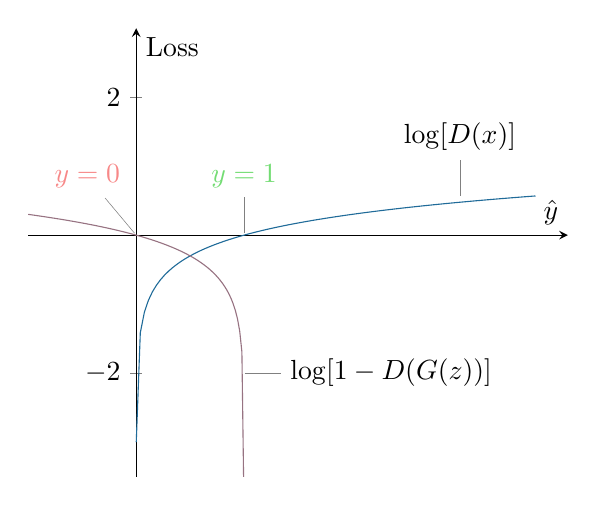
\begin{tikzpicture}
        \begin{axis}[
          axis lines=middle,
          samples=100, xmajorticks=false,
          ymax=3,
          ymin=-3.5,
          xmax=4,
          xlabel={$\hat{y}$},
          ylabel={Loss}
        ]
        \addplot[blu2,domain=0.001:3.7] {log10(x)};
        \addplot[plumb!70!gray,domain=-1:1] {log10(1-x)};
        \node[pin={90:$\log [D(x)]$},inner sep=0pt] 
          at (axis cs:{3,log10(3.5)}) {};
        \node[pin={0:$\log[1-D(G(z))]$},inner sep=0pt] 
          at (axis cs:{0.99,-2}) {};
        \node[pin={100:\textcolor{red1}{\textbf{$y=0$}}},inner sep=0pt]
          at (axis cs:{0,0}) {};
        \node[pin={90:\textcolor{gren2}{\textbf{$y=1$}}},inner sep=0pt]
          at (axis cs:{1,0}) {};
        \end{axis}
    \end{tikzpicture}
    \caption*{Equations \ref{eq:spade} and \ref{eq:club}}
\end{wrapfigure}
since the label given to real data is $1$, loss in classifying real data from $\textbf{X}$ is 
\begin{equation}
        L(D(x),1) = \log[D(x)] \label{eq:spade}.
\end{equation}
Similarly, with fake data being labeled $0$, error in its classification is given by
\begin{equation} \label{eq:club}
    L(D(G(z),0) = \log[1-D(G(z))].
\end{equation}
\\ As can be seen graphically, $D$ \emph{minimises} loss by \emph{maximising} equations \ref{eq:spade} and \ref{eq:club}, thus being as close as possible to correctly predicting 1 for real molecules, and 0 for fake molecules. $G$ wants to minimise equation \ref{eq:club}, maximising the probability of $D$ making an incorrect prediction. As a result, $D$ and $G$ play a minimax game (a term borrowed from game theory meaning the \emph{minimum} loss that can be guaranteed in a \emph{maximum} loss scenario, or the best score a player can get assuming the other player will play the best move). We arrive at equtaion \ref{eq:gan}, the learning criterion for a GAN stated in the original paper\cite{goodfellow_generative_2014}.
\begin{equation}\label{eq:gan}
\min_G\max_D[\mathbb{E}_{x \sim p_d(x)}\log(D(x)) + \mathbb{E}_{z \sim p_z(z)}\log(1-D(G(z)))]. 
\end{equation}
Convergence is reached when the discriminator consistently outputs 0.5 (this is proven mathematically to be the minimax game solution in appendix \ref{app:Dop}), as it cannot distinguish real from fake. At this point, equations \ref{eq:spade} and \ref{eq:club} both converge to $\log{0.5} \approx -0.6931$. In the actual implementation, we minimise the negative of the cost function for $D$, rather than maximising, thus our convergence is at $log(2) \approx 0.6931$
\pagebreak
%%%%%%%%%%%%%%%%%%% Results %%%%%%%%%%%%%%%%%%%%%%%%%
\section{Results and discussion}
%Talk about normalising data
\subsection{Optimal Atomic Arrangement (script \ref{code:optim})} \label{subsec:optimal}
We take three distinct atoms whose interaction is approximated by the Lennard-Jones potential. The configuration that corresponds to minimum energy is found by means of a gradient descent optimisation algorithm. A python script randomly generates an initial three atomic positions, evaluates the energy with the following definition via Lennard-Jones, where $r_{ij}$ is the distance between atoms $i$ and $j$,
\begin{equation}
    E = E_{12} + E_{13} +  E_{23}
\end{equation}
and
\begin{equation}
    E_{ij} = \epsilon \left[ \left(\frac{r_0}{r_{ij}}\right)^{12} - \left(\frac{r_0}{r_{ij}}\right)^6 \right].
\end{equation}
We then update their positions to minimise energy via a method of steepest descent (updating the position in the direction of steepest energy decrease, detailed in appendix \ref{app:gradient}). The global minimum of the energy phase space surface is shown below. First, represent the atom with one atom always fixed at the origin, and another always on the x-axis. This leaves three degrees of freedom. Another script performs the same operation but each atoms 2D Cartesian coordinate may vary.
%  First  two  triangles
\begin{figure}[ht]
\centering
\begin{subfigure}[t]{0.45\textwidth}
   \includegraphics[width = \linewidth]{images/triangle1.eps}
    \caption{Three coordinate representation}
    \label{fig:tri3}
\end{subfigure}
\begin{subfigure}[t]{0.45\textwidth}
   \includegraphics[width = \linewidth]{images/triangle2.eps}
    \caption{Six coordinate representation}
    \label{fig:tri6}
\end{subfigure}
\caption{Atomic arrangement for three atoms interacting via a Lennard - Jones potential. In \ref{fig:tri3} The molecules are defined to have one atom fixed at the origin, and a second fixed to the x-axis. Giving in general $n-3$ degrees of freedom, with $n$ atoms in a molecule. In \ref{fig:tri6} we allow now for all $2n$ Cartesian coordinates to vary. Energy for this molecule is determined to be -7.5 (units depending on parameters chosen for $\epsilon$ and $R_0$ in Lennard-Jones)}
\label{fig:Optimaltri}
\end{figure}
%%%%%
\subsection{Generating Data (script \ref{code:data})} \label{subsec:generate}
Once the minimum energy molecule is determined, it was used to create a database of similarly shaped molecules. Each coordinate in both the three and six coordinate parameterisations were extended to form a distribution of coordinates centred at the optimal molecule. Both normal and uniform distributions were tested in the remainder of the experiments. For normal distribution, variance of 0.05 was used. For uniform distribution, a range of $\pm 0.15$ was used. Energies for each of these sample molecules were also recorded via Lennard-Jones.
%
\subsection{Predict Energies (script \ref{code:net1})} \label{subsec:nrg}
Using the Keras\cite{noauthor_keras_nodate} machine learning library for Python, a series of neural networks were constructed that can predict the energy of a molecule from the distribution described in subsection \ref{subsec:generate}. Successful results were obtained for both normally distributed, and uniform training data. Results are shown in figures \ref{fig:Net1}, \ref{fig:Net2} and \ref{fig:Net3}. The resultant mean average error (MAE) is given in each plot title. A notable result here is that standardising data to a zero centered, unit variance Gaussian distribution via a linear transoformation 
\begin{equation*}
    \Tilde{\textbf{X}} = \frac {\textbf{X} - mean(\textbf{X})} {std.dev(\textbf{X})}
\end{equation*}
drastically improved model accuracy. This was done to all data before training.
%% Net 1
\begin{figure}[h!]
\centering
    \begin{subfigure}[t]{0.49\textwidth}
        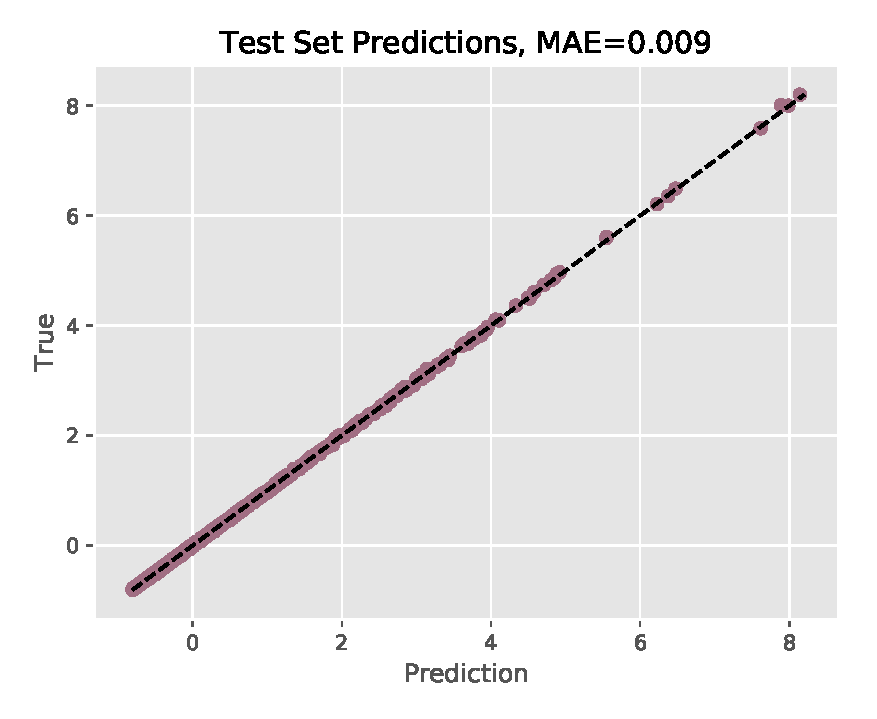
\includegraphics[width = \linewidth]{images/prediction1.eps}
        \caption{Accuracy}
        \label{fig:3acc}
    \end{subfigure}
    \begin{subfigure}[t]{0.49\textwidth}
        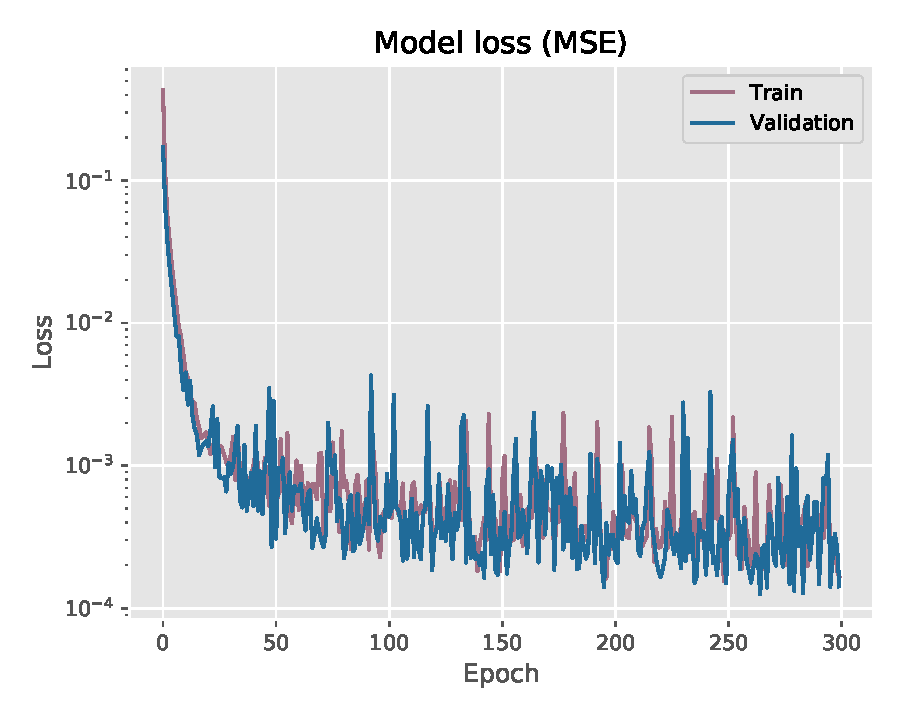
\includegraphics[width = \linewidth]{images/loss1.eps}
        \caption{Learning Curve}
        \label{fig:3loss}
    \end{subfigure}
\caption{Figure \ref{fig:3acc} shows the performance of a network trained on data with three coordinate parameterisation. The accuracy shows that the NN has adequately learned a function to predict energy with good accuracy. Both training and validation error decrease consistently in \ref{fig:3loss}, indicating no overfitting. This is unsurprising due to the relatively simple function that is being approximated. The minimum energy found in \ref{subsec:optimal} was -7.5, so MAE of 0.009 corresponds to a 0.12\% error.}
\label{fig:Net1}
\end{figure}
%%Net 2
\begin{figure}[h!]
\centering
    \begin{subfigure}[t]{0.49\textwidth}
        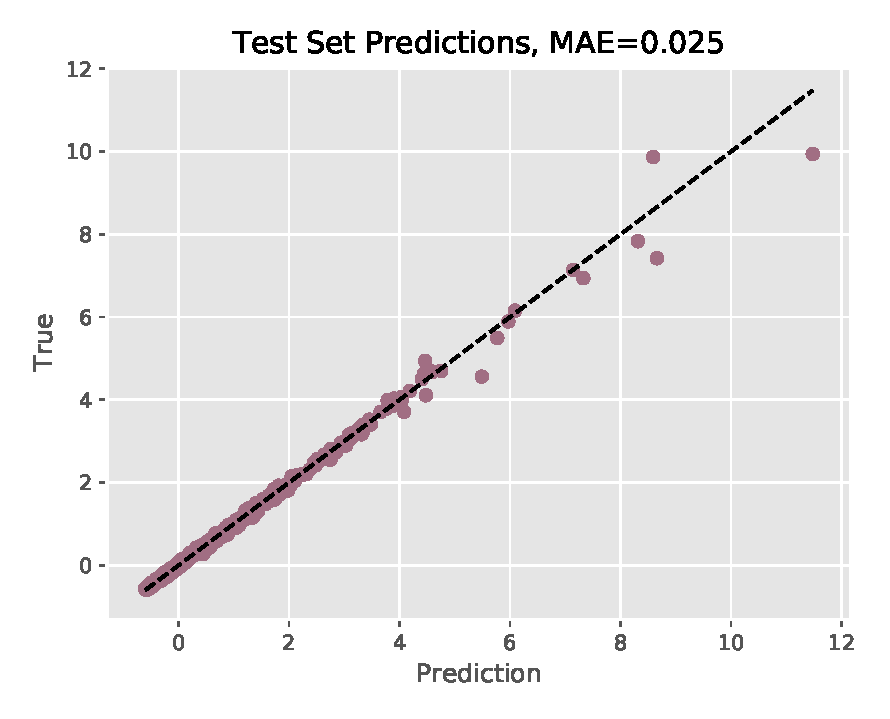
\includegraphics[width = \linewidth]{images/prediction2.eps}
        \caption{Accuracy}
        \label{fig:6acc}
    \end{subfigure}
    \begin{subfigure}[t]{0.49\textwidth}
        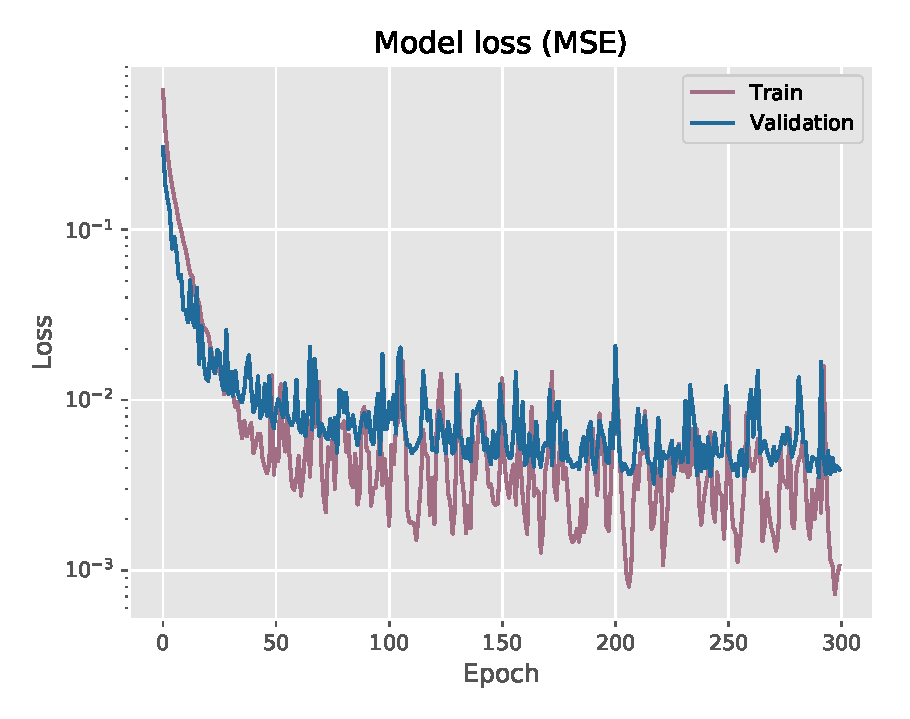
\includegraphics[width = \linewidth]{images/loss2.eps}
        \caption{Learning Curve}
        \label{fig:6loss}
    \end{subfigure}
\caption{Figure \ref{fig:6acc} shows a network trained with six coordinate data. The network again succesfully predicts energy albeit with less accuracy. Validation loss is below training loss consistently, indicating some minor overfitting. Clearly, doubling the number of independent input variables notably impairs model performance, as MAE increases from $0.009$ to $0.025$. For data like this, it would be beneficial to perform a data transformation to three coordinate representation.}
\label{fig:Net2}
\pagebreak[4]
\end{figure}
%%Net 3
\begin{figure}[h!]
\centering
    \begin{subfigure}[t]{0.49\textwidth}
        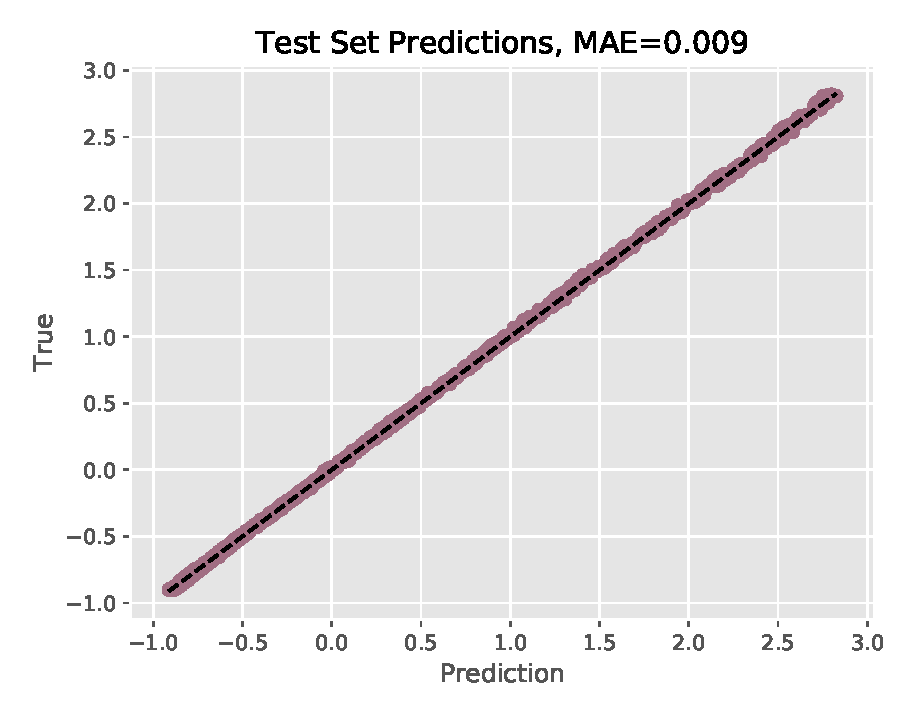
\includegraphics[width = \linewidth]{images/prediction3.eps}
        \caption{Accuracy}
        \label{fig:distacc}
    \end{subfigure}
    \begin{subfigure}[t]{0.49\textwidth}
        \includegraphics[width = \linewidth]{images/loss3.eps}
        \caption{Learning Curve}
        \label{fig:distloss}
    \end{subfigure}
\caption{The third network, trains on molecules represented simply as a list of interatomic distances. Seeing as this is the same number of independent inputs, it is unsurprising that we obtain similar results to the first network in figure \ref{fig:Net1}, with MAE again equal to $0.009$ Reconstructing the atom from this data is not trivial, and is known as the molecular distance geometry problem. This is discussed in appendix \ref{app:molecular}. For this reason, it is probably preferable to use the three coordinate Cartesian representation, at least for a three atom molecule in 2D. The only notable advantage here is that the model appears to train significantly faster, with the same error taking 300 epochs for the Cartesian, but only 30 for the interatomic.}
\label{fig:Net3}
\pagebreak
\end{figure}
\subsection{Data Transformation (script \ref{code:trans})} \label{subsec:trans}
Data were read in six coordinate Cartesian form and transformed to the reduced Cartesian case with three degrees of freedom. This was done by translating one atom to the origin and then rotating so that a second atom lies on the x axis. Result of this transformation is shown in figure \ref{fig:transformation}. Once this is applied, all neural networks can be trained to learn only three coordinates such as the one in figure \ref{fig:Net1}. This is in practice less computationally expensive and more efficient to train. The transformed data were used to compare the three networks in section \ref{subsec:nrg}.

Similarly, a trivial script can be used to turn Cartesian into representation into interatomic distance representation, to allow use of the network in figure \ref{fig:Net3}. Due to the added complication of the molecular distance geometry problem (see appendix \ref{app:molecular}), we stick to the three coordinate Cartesian representation.
\begin{figure}[h!]
    \centering
    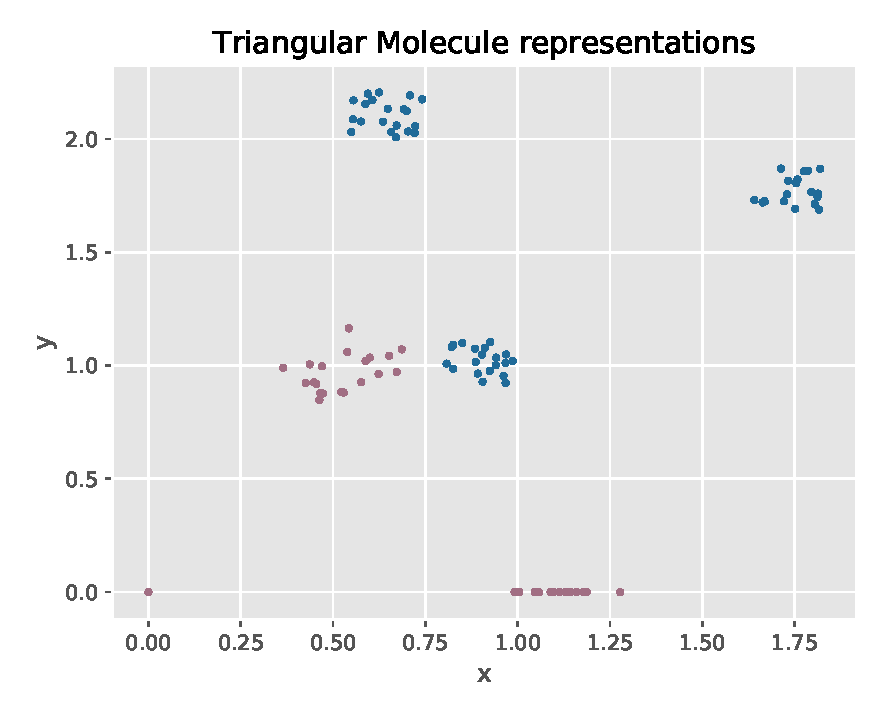
\includegraphics[width = 0.5\linewidth]{images/transformation.eps}
    \caption{Representation of molecules before and after the data transformation is applied. Blue dots indicate atomic positions for atoms in the \emph{six} coordinate Cartesian representation $\{(x_1,y_1), (x_2,y_2), (x_3,y_3)\}$, while purple dots indicate the transformed data to \emph{three} coordinates $\{(0,0), (x_2,0), (x_3,y_3)\}$. After applying this transformation, better neural network and subsequently, better GAN results can be obtained due to its simplification. Performing this transformation also has the added benefit of reducing the need for a NN or GAN to know anything about translated or rotated molecules, since they are physically equivalent we may discard this information in training.}
    \label{fig:transformation}
    \pagebreak
\end{figure}
% \subsection{Symmetries of Coordinate representations}
% \textcolor{red1}{predictions made by a trained model after transforming a molecule.  Compare results for parameterisations. Don't think this will work, hasn't so far anyway}

\clearpage
\subsection{Predicting Energy for Different Molecules} %\ref{code:shapes}
With three atoms, the global minimum for the potential energy surface corresponds to an equilateral triangle, as was numerically confirmed in section \ref{subsec:optimal}. However, the gradient descent algorithm may also find another \emph{local} minimum where an atomic arrangement might form a quasi-stable molecule. This is the case for three collinear atoms. Using this result, a second dataset consisting of atoms close to a linear arrangement was created. This was used to test the neural network's ability to learn the energy for two differently shaped molecules simultaneously. 
\begin{figure}[!h]
\centering
\begin{subfigure}[t]{0.49\textwidth}    
    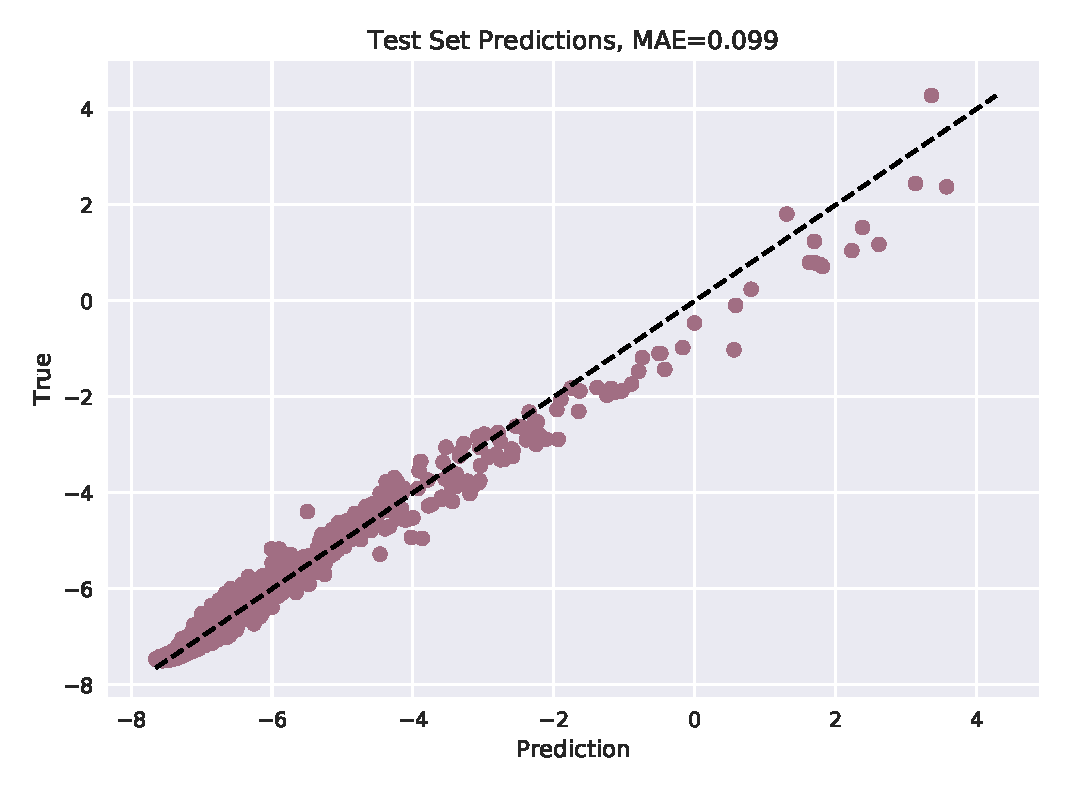
\includegraphics[width = \linewidth]{images/predictionshapes.eps}
    \caption{Accuracy}
    \label{fig:5sub1}
\end{subfigure}
\begin{subfigure}[t]{0.49\textwidth}
    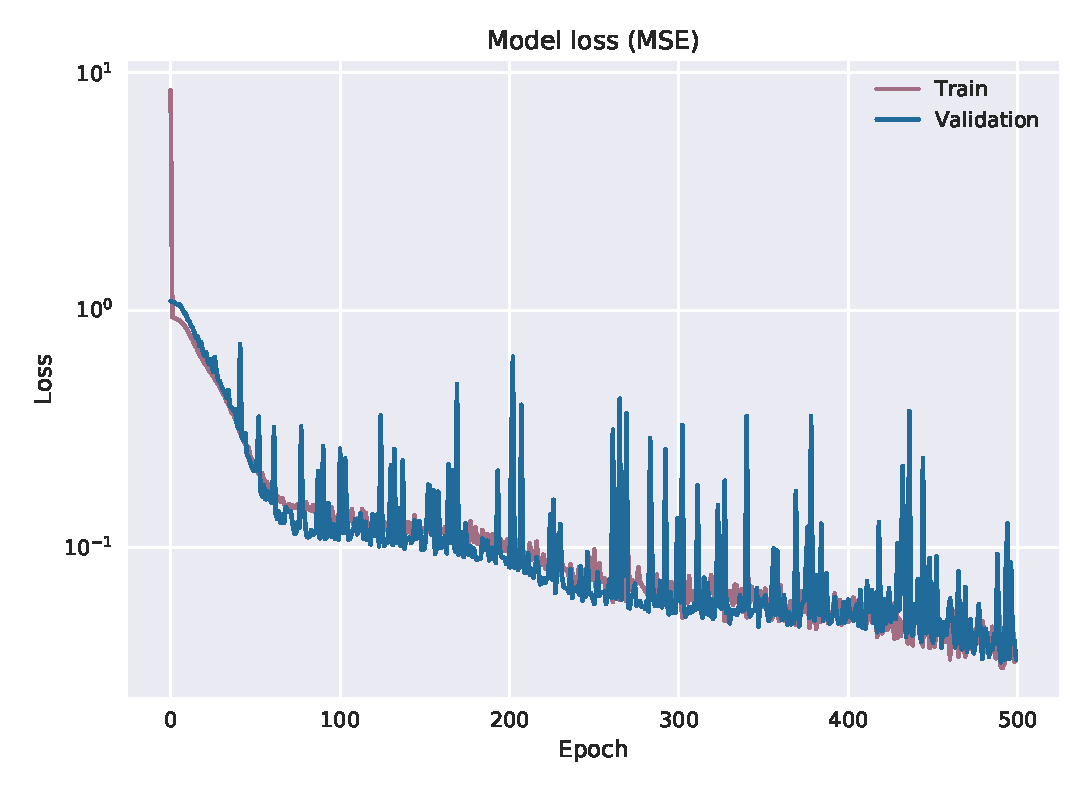
\includegraphics[width = \linewidth]{images/lossshapes.eps}
    \caption{Loss}
    \label{fig:5sub2}
\end{subfigure}
\caption{Energy predictions from a network trained on two distinctly shaped molecules, an atom of three collinear atoms and a trigonal planar arrangement. After a significantly greater period of training, the network is able to correctly predict energy. Albeit with less accuracy than the single molecule network, we find MAE is approximately ten times the case of the two most succseful networks (\ref{fig:Net1} and \ref{fig:Net3})}
\label{fig:shapes}
\end{figure}
%
\subsection{GAN (script \ref{code:gan3})}
The following are results of a Generative Adversarial network (GAN). GANs were created using the PyTorch \cite{noauthor_pytorch_nodate} library for python which allows for deeper customisation than Keras but trickier coding. Again we compare performance for the three coordinate and six coordinate representations. The aim is to create trigonal molecues identical to those in the training set. In all cases, it was noted GANs were far more capable of modelling Gaussian $p_d(x)$ than uniform. The latter is displayed in all results below. 
%%%%% GAN3
\begin{figure}[!h]
\centering
\begin{subfigure}[t]{0.49\textwidth}
    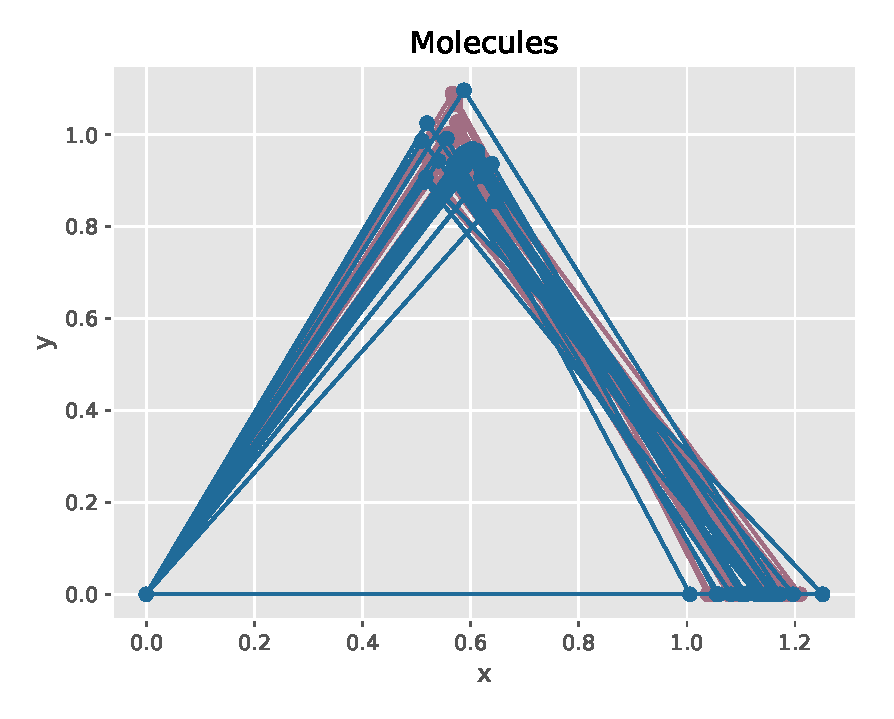
\includegraphics[width = \linewidth]{images/gan3.eps}
    \caption{Output}
    \label{fig:gan3mols}
\end{subfigure}
\begin{subfigure}[t]{0.49\textwidth}
    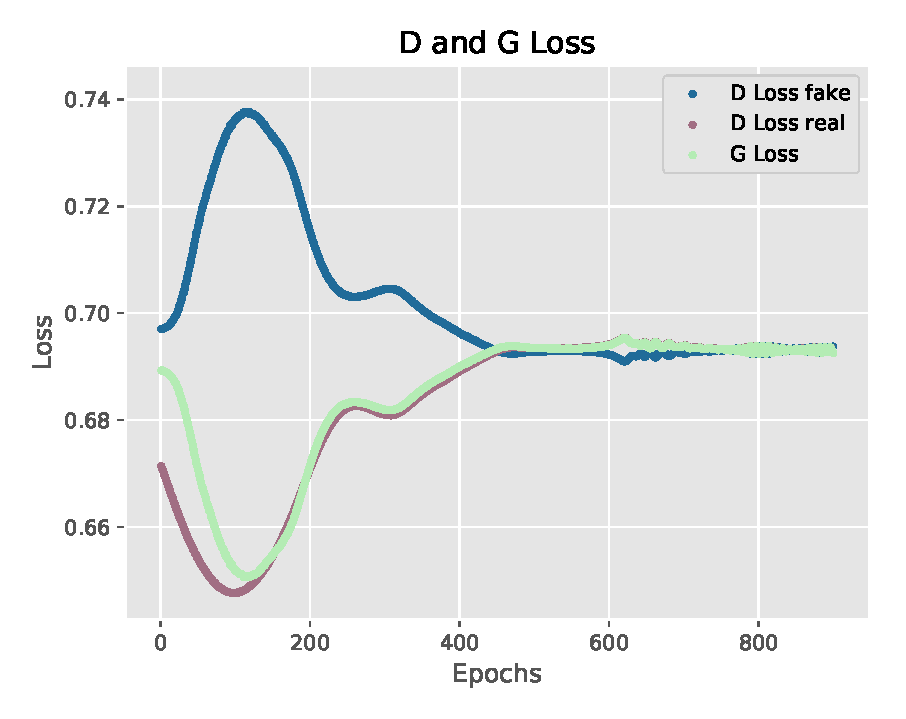
\includegraphics[width = \linewidth]{images/gan3loss.eps}
    \caption{Loss}
    \label{fig:gan3loss}
\end{subfigure}
\caption{A GAN is trained to generate trigonal homonuclear molecules indistinguishable from those it is trained on. A sample of real molecules (\textcolor{blu2}{blue}) and molecules generated by the three coordinate GAN (\textcolor{plumb}{purple}) are shown. \ref{fig:gan3loss} is model loss. The three curves represent $D$ loss in identifying real molecules, $D$ loss in identifying fake molecules, and $G$ loss in fooling $D$}
\label{fig:gan3}
\end{figure}
%%%%% GAN6
\begin{figure}[h!]
\centering
\begin{subfigure}[t]{0.49\textwidth}
    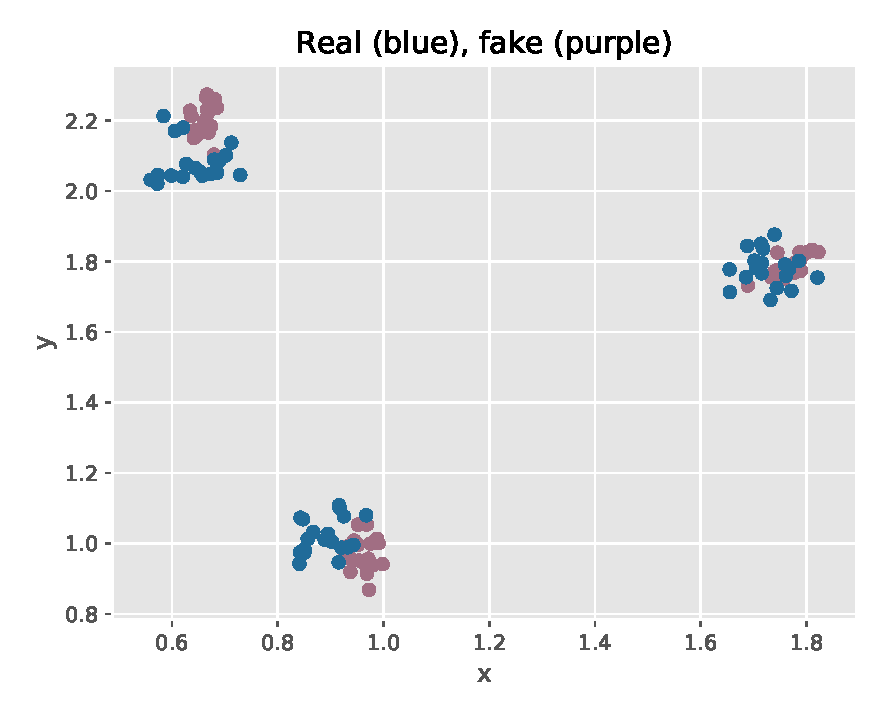
\includegraphics[width = \linewidth]{images/gan6.eps}
    \caption{Output}
    \label{fig:gan6mols}
\end{subfigure}
\begin{subfigure}[t]{0.49\textwidth}
    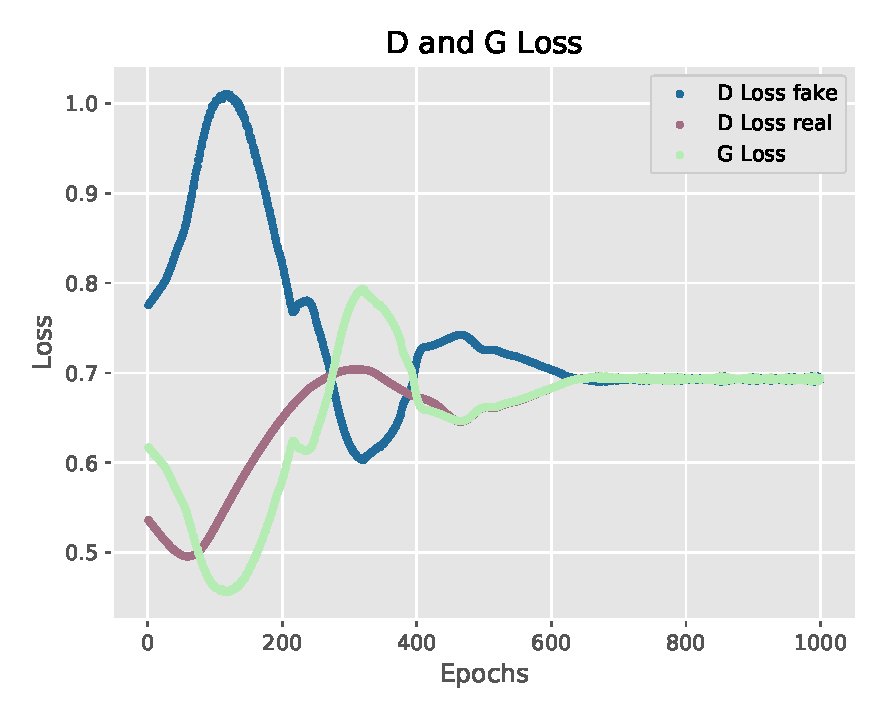
\includegraphics[width = \linewidth]{images/gan6loss.eps}
    \caption{Loss}
    \label{fig:gan6loss}
\end{subfigure}
\caption{A GAN is trained to generate trigonal homonuclear molecules indistinguishable from those it is trained on.  Sample of real molecules (\textcolor{blu2}{blue}) vs. molecules generated by the three coordinate GAN (\textcolor{plumb}{purple}). This time it generates a full six coordinates, three components of loss are the sameas in \ref{fig:gan3loss}.}
\label{fig:gan6}
\end{figure}

\clearpage
A well trained GAN, as described by Goodfellow\cite{goodfellow_generative_2014}, will not just reproduce singular results that look like they are from the training data. It will produce a \emph{distribution} of fake data indistinguishable from its training distribution. In order then to examine its efficacy, we must look deeper than a sample of fake molecules, and instead compare $p_g(z)$, the distribution from $G$, to the training distribution $p_d(x)$. This is shown in \ref{fig:gan3dist} for the three coordinate GAN and \ref{fig:gan6dist} for the six coordinate one.
\begin{figure}[h!]
    \centering
    \begin{subfigure}[h]{0.50\textwidth}
        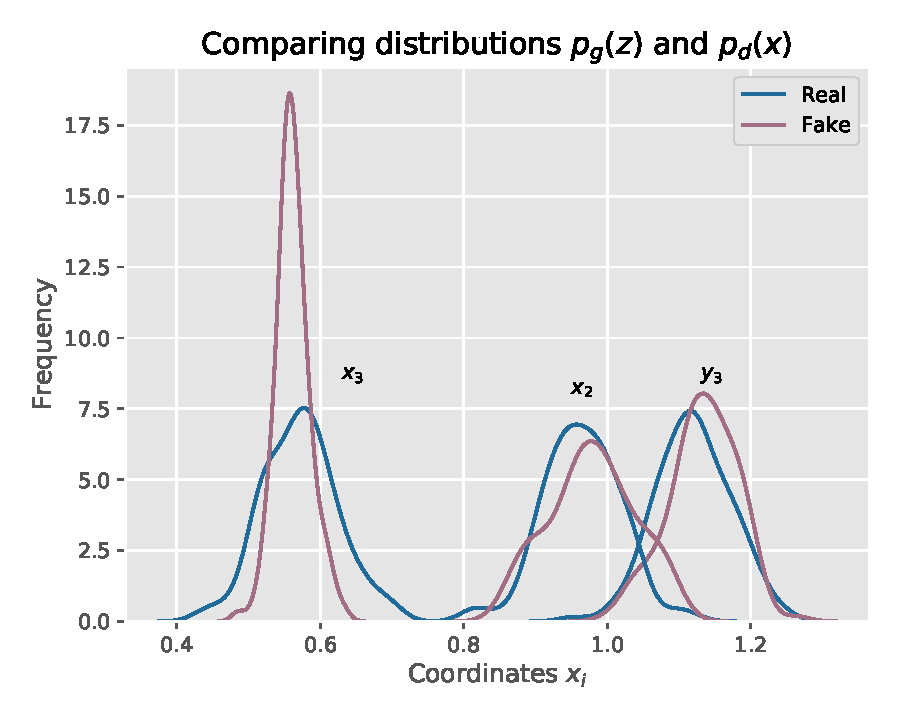
\includegraphics[width = \linewidth]{images/gan3distrib.eps}
        \caption{Three coordinate Cartesian}
        \label{fig:gan3dist}    
    \end{subfigure}
    \hspace{-0.28cm}
    \begin{subfigure}[h]{0.50\textwidth}
        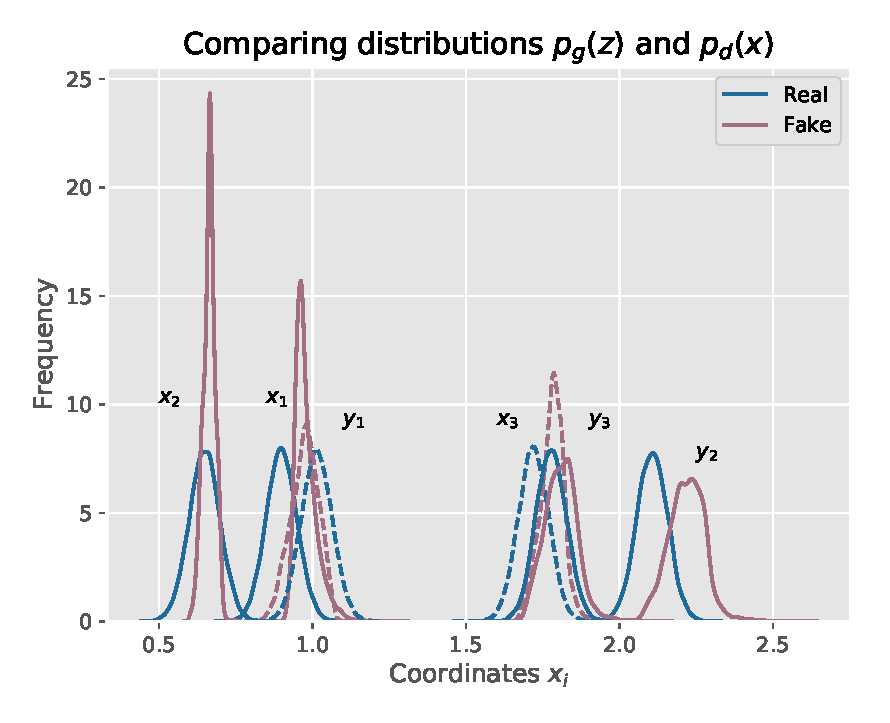
\includegraphics[width = \linewidth]{images/gan6distrib.eps}
        \caption{Six coordinate Cartesian}
        \label{fig:gan6dist}    
    \end{subfigure}    
\caption{The GAN attempts to reproduce the distribution of the real data. In the case of \ref{fig:gan3dist}, that means three distinct Gaussian curves to replicate. We find the mean is in the right position for each coordinate, and the variance is right for $x_2$ and $y_3$, but slightly too narrow for $x_3$ (this is evident in figure \ref{fig:gan3mols}). For the GAN in \ref{fig:gan6dist}, there are six Gaussians to reproduce. We find variance too narrow for fake $x_1, x_2$ and $x_3$ with mean slightly right-skewed for $y_3$. In order for the GAN to be fully accurate, these distributions should be identical. We see good results in both representations, but better for the three coordinate representation. This is another argument for the transformation described in section \ref{subsec:trans}}.
\end{figure}
%
\pagebreak
\subsection{Wasserstein GAN}
The original \enquote{vanilla} GAN is prone to several downfalls, one of these is a failure known as mode collapse. $G$ fools the generator, but then consistently outputs the same thing since it knows what works, resulting in no diversity in $p_g(x)$. There are several variations on the original GAN, one of which is the Wasserstein GAN (WGAN) \cite{arjovsky_wasserstein_2017}. The WGAN remedies mode collapse and has the added benefit of more stable learning.  A WGAN was made with some adjustments to the GAN from \autoref{fig:gan3mols}. The exact changes are commented in code \ref{code:gan3}.

\begin{figure}[h!]
    \centering
    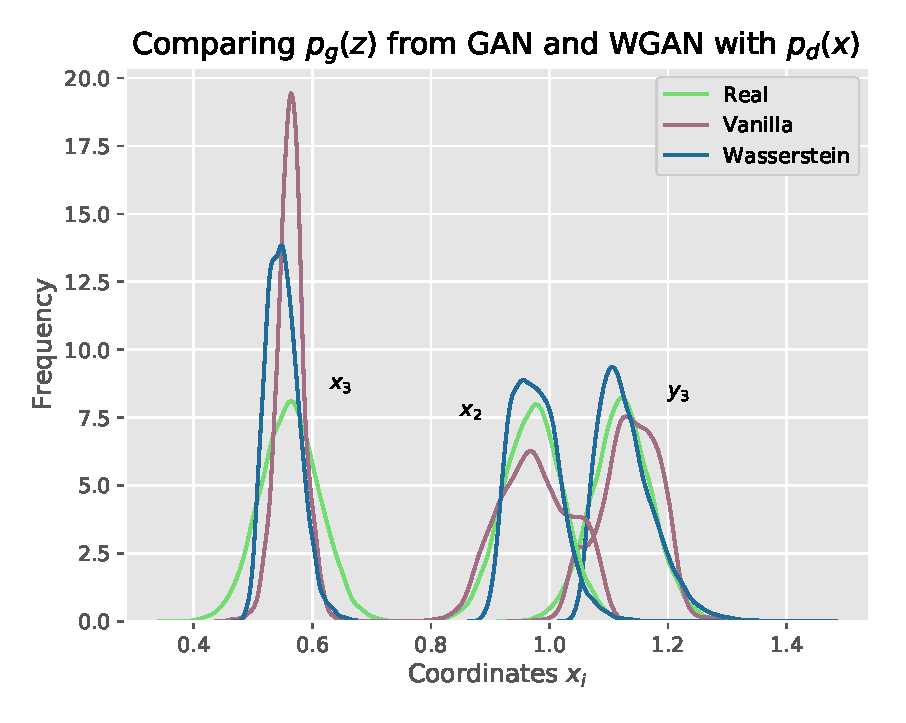
\includegraphics[width=0.5\textwidth]{images/wazzer.eps}
    \caption{Output of a WGAN \cite{arjovsky_wasserstein_2017}, compared to that of the original \emph{\enquote{vanilla}} GAN proposed by Goodfellow \cite{goodfellow_generative_2014}. Results are significantly better, with less mode collapse (wider distribution) on $x_3$, and almost perfect reproduction for $x_2$ and $y_3$ }
    \label{fig:transformation}
\end{figure}
% , namely
% \begin{itemize}
%     \item Switching to \emph{mean absolute difference loss}
%     \item Removing the sigmoid activation function from $D$
%     \item Clipping weights in $D$
%     \item Changing optimiser from \emph{Adam} to RMSprop
%     \item Lowering the learning rate, and training $D$ more than $G$
% \end{itemize}
% \subsection{Latent space heat map of real molecules}
% \textcolor{red1}{need to do this}
\section{Conclusion}
In summary, the implementation of deep learning methods was explored in the context of molecular properties. This can be a quick and efficient way to probe new material concepts. Neural networks were successfully used to give molecular energy predictions, while GANs were used as generators of \emph{fake} molecules.

A salient point is the importance of processing input data before training any ML program. In the case of the NN, by simply standardising the data to be a zero centered, unit variance distribution, we obtain far more accurate results. Since this is a linear, and therefore invertible operation, recovering the real space molecule from transformed data is trivial. In the context of NN and GAN, it was found that transforming data from six Cartesian coordinates to a reduced representation, either by fixing an atom at the origin, and another on the x axis, or by simply recording interatomic distances. Both are useful for eliminating differences up to a symmetry, i.e. treating two rotated or translated molecules as the same one. The former reduction here is preferable, since converting to distances effectively loses information, and requires complex numerical methods concerned with the molecular distance geometry problem (appendix \ref{app:molecular}) to recover.

In practice, there are many complexities to training a NN or a GAN. Finding good results relied on trying many different architectures, optimisers, loss functions, learning rates and training lengths - to name but a few changeable parameters. Networks are a black box, and for that reason tricky to troubleshoot or improve. WGAN is one of many potential variants of a GAN that can help overcome issues with training. One attempt at peering inside the black box was to map what sections of latent space $p_z(z)$ corresponded to real molecules. Unfortunately this yielded no illuminating results.

The next logical step would be to scale up to an arbitrary number $n$ of atoms in a molecule. The reduced Cartesian parameterisation would have in general $2n-3$ independent components, while the interatomic distance one would have $n \choose 2$ possible interatomic distances to consider. This of course scales far more quickly than $2n-2$, and for any greater than five atoms, would be even worse than $2n$ Cartesian coordinates with no reduction. It is possible that not all interatomic distances would be required, reducing this number, or that applying other known information about atoms could help infer bond angles and shapes,or  perhaps knowing only \emph{some} interatomic distances would suffice in some contexts.

The limitations of this study lie with the diversity of molecules examined. In theory, it would not be difficult to extend to three dimensions, and introduce more complex molecules with different atoms, we should then use something other than Lennard-Jones potential, which was really designed only species such as argon \cite{Lennard_Jones_1931}. Once adequate methods of training ML models are determined, they can be made with more inputs and applied to new data. We could easily upgrade the models shown here to homonuclear molecules with more atoms.

With effective programming, these methods could be combined to design molecules with desired properties. GANs could generate new molecules, whose \enquote{realness} would be their chemical viability. Neural networks could work to simultaneously determine properties of the molecule, and matched to desired ones. All of this could be combined into the integrated feedback loop of inverse design, proposed by Sanchez-Lengeling \cite{sanchez-lengeling_inverse_2018}.

\printbibliography[]

\section{Appendices}
% \subsection{Supplementary}
\subsection{Gradient Descent} \label{app:gradient}
\begin{wrapfigure}{r}{0.3\textwidth}
\vspace{-1cm}
    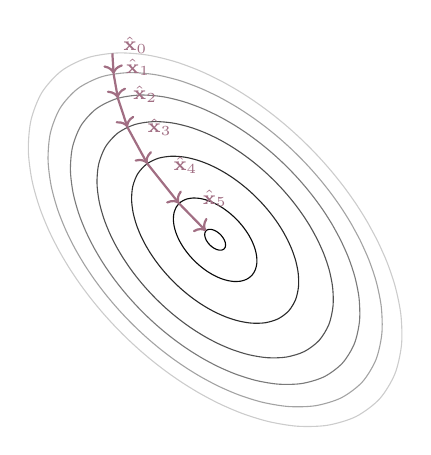
\begin{tikzpicture}[samples=50,smooth,scale=0.65]
            %\clip(-4,-1) rectangle (4,4);
            \path[bend left,name path=arrowcurve] (-2,4) to[out=-30,in=-160] (0,0);
            \foreach \y[count=\i] in {20,16,12,8,4,1,0.0625}{
            \pgfmathsetmacro\colper{\y*4} % color percentage variable
                \draw[name path global/.expanded=curve\i,white!\colper!black] plot[domain=0:360] ({cos(\x)*sqrt(\y/(sin(2*\x)+2))},{sin(\x)*sqrt(\y/(sin(2*\x)+2))});
                \draw[name intersections = {of ={curve\i} and arrowcurve}](intersection-1) coordinate (P\i);
                \ifnum\i=1 
                    % do nothing
                \else%
                    \pgfmathtruncatemacro\imin{\i-1}
                    \pgfmathtruncatemacro\iprint{\i-2}
                    \draw[->, plumb, thick] (P\imin) -- (P\i) node[above right,midway] {\scriptsize $\hat{\textbf{x}}_{\iprint}$}; 
                \fi%
            }     
    \end{tikzpicture}
\caption*{\centering Gradient descent on a series of level sets}
\end{wrapfigure}
Gradient descent is an iterative algorithm ubiquitous in numerical optimisation. It was first proposed by Augustin-Louis Cauchy  \cite{lemarechal_cauchy_2012}. The algorithm is used to find minima of a multivariable function $F$. To do this, we take steps in the direction of the negative of the gradient of the function at a given point.
a sequence $\textbf{x}_i$ will converge to a minimum provided
\begin{equation}
    \textbf{x}_{n+1} = \textbf{x}_n - \epsilon \nabla F(\textbf{x}_n).
\end{equation}
\subsection{The Molecular Distance Geometry Problem} \label{app:molecular}
Distance geometry is a branch of topology concerning the study of sets given only distances between their points, in other words, it is the study of \emph{semimetric spaces}. This is important for chemists studying molecular shapes, as there are methods, such as nanomagnetic resonance imaging, to find distances between atoms. The task is then to recover the shape of the molecule from this data. In general, various different numerical algorithms are employed for this purpose \cite{liberti_molecular_2011} which will not be discussed here. 
\subsection{GAN is optimised for D(x) outputting 0.5 \cite{goodfellow_generative_2014}}\label{app:Dop}

There is unique solution to the minimax game (equation \ref{eq:gan}) corresponding to $p_g(z)=p_d(x)$
\begin{proof}
Begin with equation \ref{eq:ganrad}, which comes from the Radon-Nikodym theorem of measure theory. The theorem concerns finding the expected value of a function $f$ of a random variable $x$ when the probability distribution of $x$ is known, but that of $f$ is not. here it is applied to the unknown distribution $p_g(z)$ and the known distribution $p_d(x)$.
\begin{equation}\label{eq:ganrad}
\mathbb{E}_{z \sim p_z(z)}\log(1-D(G(z)))  = \mathbb{E}_{x \sim p_g(x)}\log(D(x)). 
\end{equation}
This can be rewritten
\begin{equation} \label{eq:a}
\begin{split}
&\int_xp_d(x)\log D(x) \text{d} x + \int_zp(z)\log(1-D(G(z))) \text{d} z\\
=&\int_xp_d(x)\log D(x) + p_g(x)\log(1-D(x)) \text{d}x \cite{goodfellow_generative_2014}.
\end{split}
\end{equation}
The optimal $D$ for a given $G$ is given by maximising the integrand of equation \ref{eq:a}. This can be done easily by (for simplicity letting $a =p_d(x)$ and $b=p_g(x)$) writing it as
\begin{equation}
    f(y) = a\log y + b\log (1-y),
\end{equation}
and solving 
\begin{equation}
    f'(y) = 0 \implies \frac ay - \frac{b}{1-y} = 0 \implies y = \frac{a}{a+b}.
\end{equation}
Further demonstrate that if $a+b \ne 0$, this is a maximum by taking second derivative,
\begin{equation}
    f''(\frac{a}{a+b}) =-\frac{a}{\left(\frac{a}{a+b}\right)^2}-\frac{b}{\left(1-\frac{a}{a+b}\right)^2} < 0 
\end{equation}
This implies that the optimal value of $D(x)$ corresponding to a maximum value of the minimax value function (integrand in equation \ref{eq:a}) is given by
\begin{equation}
    D(x) = \frac{p_d(x)}{p_d(x)+p_g(z)}
\end{equation}
Recalling we require $p_g(z)=p_d(x)$ at the theoretical convergence, plugging into optimal value for D(x) we get the output of 0.5.
\end{proof}
%%%%%%%%%%%%%%%%%
\clearpage
\section{Code}
\subsubsection{Determine Optimal atomic arrangement} \label{code:optim}
\begin{lstlisting}
# Determine forces on particles as the Gradient of the of Lennard-Jones potential Hypersurface
def F2x(x2,x3,y3):
    return e*((-12*R0**12 *x2**-13) + (6*R0**6 *x2**-7) + (12*R0**12 *(x3-x2)*((x3-x2)**2+y3**2)**-7) + (-6*(x3-x2)*R0**6*((x3-x2)**2+y3**2)**-4))
def F3x(x2,x3,y3):
    return e*((-12*R0**12*(x3)*(x3**2+y3**2)**-7) + (6*x3*R0**6*(x3**2+y3**2)**-4) +  (-12*R0**12*(x3-x2)*((x3-x2)**2+y3**2)**-7) + (6*R0**6*(x3-x2)*((x3-x2)**2+y3**2)**-4))
def F3y(x2,x3,y3):
    return e*((-12*R0**12*y3*(x3**2+y3**2)**-7) + (6*y3*R0**6*(x3**2+y3**2)**-4) + (-12*R0**12*y3*((x3-x2)**2+y3**2)**-7) + (6*R0**6*y3*((x3-x2)**2+y3**2)**-4))

d = 0.01
error = 0.00000001

def F(F2x, F3x, F3y): # Total Force on particles
    return np.abs(F2x) + np.abs(F3x) + np.abs(F3y)

iterations = 0
while F(F2x(x2var, x3var, y3var), F3x(x2var, x3var, y3var), F3y(x2var, x3var, y3var)) > error :
    x2var += -F2x(x2var, x3var, y3var) * d
    x3var += -F3x(x2var, x3var, y3var) * d
    y3var += -F3y(x2var, x3var, y3var) * d
    iterations +=1

R12 = x2var
R13 = math.sqrt(x3var**2 + y3var**2)
R23 = math.sqrt((x3var-x2var)**2 + y3var**2)

#Keeping track of energies
E12 = e*((R0/R12)**12 - (R0/R12)**6)
E13 = e*((R0/R13)**12 - (R0/R13)**6)
E23 = e*((R0/R23)**12 - (R0/R23)**6)

E = E12 + E13 + E23
\end{lstlisting}
\subsubsection{Generate Training Data} \label{code:data}
\begin{lstlisting}
for i in range (100000):
    x2i = x2var + random.uniform(-0.15, 0.15) # returns uniform distribution
    x3i = x3var + random.uniform(-0.15, 0.15)
    y3i = y3var + random.uniform(-0.15, 0.15)
    
    x2in = np.random.normal(x2var, 0.05) # returns Gaussian distribution
    x3in = np.random.normal(x3var, 0.05)
    y3in = np.random.normal(y3var, 0.05)
    
    normal.append([x2in, x3in, y3in])
    uniform.append([x2i, x3i, y3i])
    
    R12i = x2i
    R13i = math.sqrt(x3i**2 + y3i**2)
    R23i = math.sqrt((x3i-x2i)**2 + y3i**2)
    
    E12i = e*((R0/R12i)**12 - (R0/R12i)**6)
    E13i = e*((R0/R13i)**12 - (R0/R13i)**6)
    E23i = e*((R0/R23i)**12 - (R0/R23i)**6)

    Ei = E12i + E13i + E23i
    
    R12in = x2in
    R13in = math.sqrt(x3in**2 + y3in**2)
    R23in = math.sqrt((x3in-x2in)**2 + y3in**2)
     
    E12in = e*((R0/R12in)**12 - (R0/R12in)**6)
    E13in = e*((R0/R13in)**12 - (R0/R13in)**6)
    E23in = e*((R0/R23in)**12 - (R0/R23in)**6)

    Ein = E12in + E13in + E23in
     
    nrg_uniform.append(Ei)
    nrg_normal.append(Ein)
\end{lstlisting}
\subsubsection{Three Coordinate Neural Network} \label{code:net1}
\begin{lstlisting}
# Normalise input vector
x_mu = np.mean(datalist, axis=0)
x_std = np.std(datalist, axis=0)
datalist_NORM = (datalist - x_mu)/x_std

# Normalise energies
y_mu = np.mean(nrglist)
y_std = np.std(nrglist)
nrglist_NORM = (nrglist - y_mu)/y_std

#Split into training, validation and test sets
datalist_train = datalist_NORM[:6000]
datalist_val = datalist_NORM[6000:8000]
datalist_test = datalist_NORM[8000:10000]

nrglist_train = nrglist_NORM[:6000]
nrglist_val = nrglist_NORM[6000:8000]
nrglist_test = nrglist_NORM[8000:10000]

#Create model
model = Sequential([
    Dense(64, input_shape = (3,)),
    Activation('relu'),
    Dense(32),
    Activation('relu'),
    Dense(1),
])

# Compile model
model.compile(optimizer = 'adam', loss = 'mse')

callbacks = [EarlyStopping(patience=10, verbose=1), ModelCheckpoint(save_best_only=True, verbose=1)]

# Train
epochs = 300

history = model.fit(x=datalist_train, y=nrglist_train, epochs=epochs, validation_data=(datalist_val, nrglist_val), batch_size=32,  verbose = 1, callbacks = callbacks)

#  Test Error
pred_test = model.predict(datalist_test).flatten()
mae_error = np.mean(np.abs(pred_test-nrglist_test)) # mean absolute error
print("Generalization Error (MAE): %f" % mae_error)
\end{lstlisting}
\subsubsection{Data Transformation to reduce dof} \label{code:trans}
\begin{lstlisting}
def translate(data): # translate (x1, y1) to origin, eliminating these coordinates from the parameterisation space
    translated = np.zeros((len(data), 2*N)) # N atoms
    for i in range(len(data)):
            translated[i][0] = data[i][0] - data[i][0]
            translated[i][2] = data[i][2] - data[i][0]
            translated[i][4] = data[i][4] - data[i][0]
            translated[i][1] = data[i][1] - data[i][1]
            translated[i][3] = data[i][3] - data[i][1]
            translated[i][5] = data[i][5] - data[i][1]
    return translated

def rotate(data): # rotate molecule s.t. x2 -> 0, further  reducing dof
    rotated = np.zeros((len(data), 2*N))
    for i in range (len(data)):
        y2,x2 = data[i][5],data[i][4]
        angle = np.arctan(y2/x2)
        R = np.array([[np.cos(angle), np.sin(angle)], [-np.sin(angle), np.cos(angle)]])
        p2, p3 = np.array([data[i][2], data[i][3]]), np.array([data[i][4], data[i][5]])
        p2, p3 = np.matmul(R, p2), np.matmul(R, p3)
        
        rotated[i][2] = p2[0]
        rotated[i][3] = p2[1]
        rotated[i][4] = p3[0]
        rotated[i][5] = p3[1]
    return rotated
    
new = rotate(translate(six_coord))
\end{lstlisting}
\begin{lstlisting}
def distance(data): # returns data as a list of interatomic distances
new = np.zeros((len(data), N)) # N atoms
for i in range(len(data)):
        translated[i][0] = math.sqrt((data[i][2]-data[i][0])**2+(data[i][3]-data[i][1])**2) #R12
        translated[i][1] = math.sqrt((data[i][4]-data[i][0])**2+(data[i][5]-data[i][1])**2) #R13
        translated[i][2] = math.sqrt((data[i][4]-data[i][2])**2+(data[i][5]-data[i][3])**2) #R23
return new

new = distance(six_coord)
\end{lstlisting}{}
\subsubsection{Three Coordinate GAN} \label{code:gan3}
\begin{lstlisting}
batch_size = 256
N = 3 # three atoms
Z = 4 # latent vector length

class Generator(nn.Module):
    def __init__(self, Z):
        super(Generator, self).__init__()
        self.fc1 = nn.Linear(Z, 64, bias=True)
        self.fc2 = nn.Linear(64, 64, bias=True)
        self.fc3 = nn.Linear(64, 3, bias=True) #specify three coord output
        self.act = nn.LeakyReLU()

    def forward(self, x):
        # pass through hidden layers
        x = self.act(self.fc1(x))
        x = self.act(self.fc2(x))
        x = self.fc3(x)
        return x

class Discrim(nn.Module):
    def __init__(self):
        super(Discrim, self).__init__()
        self.fc1 = nn.Linear(3, 64, bias=True) #specify 3 coord input
        self.fc2 = nn.Linear(64, 64, bias=True)
        self.fc3 = nn.Linear(64, 1, bias=True)
        self.act = nn.LeakyReLU()

    def forward(self, x):
        x = self.act(self.fc1(x))
        x = self.act(self.fc2(x))
        x = self.fc3(x)
        x = nn.Sigmoid()(x) #!!! REMOVED for Wasserstein WGAN
        return x

nn_G = Generator(Z) # Construct Networks using their generative classes
nn_D = Discrim()

criterion = nn.BCELoss() #!!! Switched to L1loss, (mean absolute difference loss)
D_op = optim.Adam(nn_D.parameters(), lr=1e-6) #!!! RMSprop optimiser used  for WGAN, learning rates also changed to same 1e-5
G_op = optim.Adam(nn_G.parameters(), lr=1e-5)

for T in range(1, epochs+1):
    cost_i = []
    for i in range(updates):
        D_op.zero_grad()

        #Load a real batch of data
        real_batch = torch.from_numpy(real(datalist, batch_size))
        output = nn_D(real_batch.float())
        D_loss_r = criterion(output, D_label_r)
        D_loss_r.backward() # computes gradient
       
#       D - Train on Fake Data
        latent_vector = torch.empty(batch_size, Z).normal_(0, 1) # latent vector, zero centred unit variance Gaussian Distribution
        fake_data = nn_G(latent_vector)
        output = nn_D(fake_data.float())
        D_loss_f = criterion(output, D_label_f)
        D_loss_f.backward()
        D_op.step()
        #for p in nn_D.parameters():  # !!! for WGAN, clamp weights to keep small
            p.data.clamp_(-0.01, 0.01)


#       G - Train
        G_op.zero_grad()
        fake_data = nn_G(latent_vector)
        output = nn_D(fake_data)
        G_loss = criterion(output, G_label)

        G_loss.backward()
        G_op.step()
\end{lstlisting}
\end{document}
